% Tamaño de letra.
\documentclass[12pt,titlepage]{article}

%------------------------------ Paquetes ----------------------------------

% Paquetes:
 
%Para comentarios multilínea.
\usepackage{verbatim}

% Para tener cabecera y pie de página con un estilo personalizado.
\usepackage{fancyhdr}

% Codificación UTF-8
\usepackage[utf8]{inputenc}

% Castellano.
\usepackage[spanish]{babel}

% Tamaño de página y márgenes.
\usepackage[a4paper,headheight=16pt,scale={0.75,0.8},hoffset=0.5cm]{geometry}

% Para poder agregar notas al pie en tablas:
%\usepackage{threeparttable}

% Tipo de letra Helvetica (Arial).
%\usepackage{helvet}
%\renewcommand\familydefault{\sfdefault}

% Gráficos:

% Para incluir imágenes, el siguiente código carga el paquete graphicx
% según se esté generando un archivo dvi o un pdf (con pdflatex).

% Para generar dv.
%\usepackage[dvips]{graphicx}

% Para generar pdf.
\usepackage[pdftex]{graphicx}
\pdfcompresslevel=9

\usepackage{appendix}
\usepackage{pdfpages}
\usepackage{longtable}
\usepackage{url}


%
% Directorio donde están las imagenes.
%
%\newcommand{\imgdir}{includes}
%\graphicspath{{\imgdir/}}

%------------------------------ ~paquetes ---------------------------------

%------------------------- Inicio del documento ---------------------------

\begin{document}

% ---------------------- Encabezado y pie de página -----------------------

% Encabezado: sección a la derecha.
% Pie de página: número de página a la derecha.

\pagestyle{fancy}
\renewcommand{\sectionmark}[1]{\markboth{}{\thesection\ \ #1}}
\lhead{}
\chead{}
\rhead{\rightmark}
\lfoot{}
\cfoot{}
\rfoot{\thepage}

% ---------------------- ~Encabezado y pie de página ----------------------

% -------------------------- Título y autor(es) ---------------------------

\title{ConcuShare}
\author{}

% -------------------------- ~Título y autor(es) --------------------------

% ------------------------------- Carátula --------------------------------

\begin{titlepage}

\thispagestyle{empty}

% Logo facultad más pie de la figura.
\begin{center}

\includegraphics[scale=0.55]{./imgs/fiuba-logo.png}\\
\large{\textsc{Universidad de Buenos Aires}}\\
\large{\textsc{Facultad De Ingeniería}}\\
\small{Año 2012 - 1\textsuperscript{er} Cuatrimestre}
\end{center}

\vfill

% Título central.
\begin{center}

\Large{\underline{\textsc{Sistema de Programaci\'on No Convencional de Robots}}}
\Large{\underline{\textsc{(75.70)}}}

\vfill

% Tabla de integrantes.

\Large{\underline{\textsc{Trabajo Pr\'actico Final}}} \\
\Large{\underline{\textsc{Utilizaci\'on de Redes Neuronales en Juegos de Ingenio}}}
\vfill
 
\Large\underline{Integrantes} \linebreak\linebreak

% Separación entre columnas.
\large\addtolength{\tabcolsep}{-3pt}
% Tres columnas con alineación centrada.
\begin{tabular}{|| c | c | c ||}
\hline
\textbf{Apellido, Nombre} & \textbf{Nro. Padrón} & \textbf{E-mail} \\
\hline
Bukaczewski, Verónica & 86954 & vero13@gmail.com \\
\hline
Rivero, Hern\'an & 88455 & riverohernanj@gmail.com \\
\hline
\end{tabular}
\end{center}

\vfill

\hrule
\vspace{0.2cm}

% Pie de página de la carátula.
%\noindent\small{75.70 - Sistema de Programaci\'on No Convencional de Robots \hfill}

\end{titlepage}

% ------------------------------- ~Carátula -------------------------------

% ----------------------- Cabeceras y pies de página ----------------------

\pagestyle{fancy}
\lhead{}
\chead{}
\rhead{}
\lfoot{\scriptsize{75.70 - Sistema de Programaci\'on No Convencional de Robots \\
\\Trabajo práctico Final - 1er cuatrimestre 2012}}
\cfoot{}
\rfoot{\\\thepage}
\renewcommand{\headrulewidth}{0pt}

% ---------------------- ~Cabeceras y pies de página ----------------------

% -------------------------------- Índice ---------------------------------

% Hago que las páginas se comiencen a contar a partir de aquí.
\setcounter{page}{2}

% Índice.
\newpage
\thispagestyle{empty}
\tableofcontents
\newpage

% -------------------------------- ~Índice --------------------------------

% ----------------------------- Inicio del tp -----------------------------

\section{Objetivo}
El objetivo del presente trabajo pr\'actico es descubrir y analizar diferentes posibilidades para entrenar una red neuronal de forma tal que sea capaz de jugar de manera eficaz a un juego de ingenio. Se utilizar\'a una red neuronal de tipo backpropagation, para generar un m\'etodo de aprendizaje a medida que se desarrollan las partidas. El juego elegido para los ensayos es el Ta-Te-Ti.

\section{El juego Ta-Te-Ti}
Por lo general, el Ta-Te-Ti se juega en una cuadrícula de tres por tres (ver Figura [\ref{grilla-vacia}]). Cada jugador, a su vez se mueve mediante la colocación de un marcador en un casillero vac\'io. El marcador de un jugador es ``X``(cruz) y el del otro es ``O``(c\'irculo). El juego termina tan pronto como un jugador tiene tres marcadores en una fila: horizontalmente, verticalmente, o en diagonal (un ejemplo se muestra en la Figura [\ref{cruz-gana}]). El juego puede también terminan en empate (ver Figura [\ref{empate-tateti}]), si no hay posibilidad de ganar para alguno de los jugadores.
Un jugador que conozca unas pocas estrategias b\'asicas puede asegurarse al menos un empate.

\begin{figure}[h!]
 \centering
 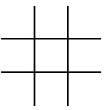
\includegraphics{./imgs/grilla-tateti.png}
 % grilla-tateti.png: 104x110 pixel, 96dpi, 2.75x2.91 cm, bb=0 0 78 82
 \caption{Grilla vac\'ia TaTeTi.}
 \label{grilla-vacia}
\end{figure}

\begin{figure}[h!]
 \centering
 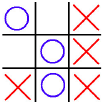
\includegraphics{./imgs/cruz-gana-tateti.png}
 % cruz-gana-tateti.png: 103x105 pixel, 96dpi, 2.72x2.78 cm, bb=0 0 77 79
 \caption{El jugador cruz gana la partida.}
 \label{cruz-gana}
\end{figure}

\begin{figure}[h!]
 \centering
 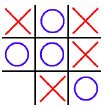
\includegraphics{./imgs/empate-tateti.png}
 % empate-tateti.png: 104x109 pixel, 96dpi, 2.75x2.88 cm, bb=0 0 78 82
 \caption{La partida termin\'o empatada.}
 \label{empate-tateti}
\end{figure}

\section{Estructura general de la soluci\'on propuesta}
Se realiz\'o un programa en lenguaje Java y se utiliz\'o el framework de red neuronal Joone. A continuaci\'on se presenta el diagrama de clases.

\begin{figure}[h!]
 \centering
 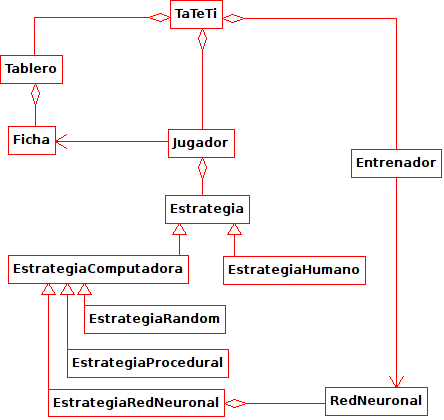
\includegraphics{./imgs/diagrama-de-clase.png}
 % diagrama-de-clase.png: 442x417 pixel, 96dpi, 11.69x11.03 cm, bb=0 0 331 313
 \caption{Diagrama de clases de la soluci\'on propuesta}
\end{figure}

\section{Soluciones propuestas}
Se armaron distintas estructuras de redes neuronales, con el objetivo de poder entrenarlas para que jueguen al Ta-Te-Ti. El primer intento fue la realizaci\'on de una red con nueve inputs y nueve outputs, al cual se le variaron la cantidad de capas ocultas. Los inputs representan los nueve casilleros del tablero y se especifican con:
\begin{itemize}
 \item 1: ficha de la red neuronal.
 \item -1: ficha rival.
 \item 0: casillero vac\'io.
\end{itemize}
Los outputs representan los nueve casillero del tablero, pero esta vez se le asocia un puntaje que nos indica que tan apropiado es jugar en dicho casillero. \\
Luego de varios intentos de aprendizaje, qued\'o descartada porque no mostraba cambios significativos al variar los inputs. 

\section{Soluci\'on utilizada}
\subsection{Estructura de la Red Neuronal}
Se arm\'o una red con dieciocho valores de input, organizados de la siguiente manera:
\begin{itemize}
 \item del 1 al 9 valen 1 si la posición está ocupada con una ficha de la red, 0 en caso contrario.
 \item del 10 al 18, valen 1 si hay una ficha del rival, 0 en caso contrario.
\end{itemize}
Los outputs son nueve y representan los puntajes para los casilleros del tablero. Se utiliz\'o una capa oculta de dieciocho filas. 

\subsection{Entrenando la Red Neuronal}
El entrenamiento de la red neuronal se realiz\'o mediante el juego contra otros algoritmos que juegan Ta-Te-Ti. Con el avance de las partidas, se le fue ense\~nando a la red neuronal los movimientos a realizar. Para ellos se utiliz\'o un sistema de puntajes donde luego de cada partida se busca que la red imite los movimientos del ganador y evite los del perdedor. De esta forma se le fue marcando un camino y con el pasar de las partidas, la red iba adquiriendo una mayor inteligencia a la hora de realizar sus jugadas. \\ 

Para analizar diferentes alternativas de entrenamiento, se construy\'o un algoritmo que sigue una estrategia met\'odica que resulta repetitiva pero efectiva y otro que simplemente coloca marcas en luga%res al azar.

\subsection{Resultados}

\pagebreak
\section{Conclusiones}
Una primera conclusi\'on nos indica que el armado de una red neuronal lleva un tiempo considerablemente mayor al del entrenamiento de la misma. Esto se debe a que el entrenamiento es un proceso automatizado, que no requiere m\'as que la configuraci\'on de algunos par\'ametros. Mientras que para el armado de una red neuronal, que nos permita resolver el problema, es necesario un conocimiento sobre la situaci\'on que
estamos enfrentando, de manera de poder crear una red que nos permita resolver el problema de manera eficiente. Por otro lado, observamos que el entrenamiento prolongado de una red mal armada no significaba llegar a los resultados deseados. Es decir, que lo m\'as importante es concentrarnos en crear una red acorde al problema; de manera de asegurarnos llegar a los resultados buscados; lo cual puede estar acompa\~nado de un tiempo de entrenamiento m\'as corto de lo esperado. \\

En cuanto a lo que se observa del entrenamiento de la red, la conclusi\'on m\'as importante que se obtiene es que no es posible alcanzar un desarrollo \'optimo si se utiliza un \'unico algoritmo. La red es capaz de aprender a defenderse del algoritmo bueno, pero esto no le va a servir al momento de enfrentarse a otros. La red aprende tambi\'en a ganarle con mucha facilidad al algoritmo aleatorio, pero utilizando estrategias muy b\'asicas que no le sirven ante un rival de mayor inteligencia. \\

La mejor forma de entrenar a la red es alternando los algoritmos que la enfrentan, de manera tal de que se encuentre con la mayor cantidad de variantes de jugadas posibles. La estrategia de jugar en posiciones aleatorias no resulta conveniente para el entrenamiento inicial. Esto es debido a que la red de esta manera, luego de una cierta cantidad de partidas, comienza a repetir siempre la misma jugada, que no necesariamente es buena pero resulta eficaz ante la nula inteligencia del rival. Prolongar un entrenamiento de estas caracter\'isticas conduce a que la red refuerce cada vez m\'as estas pr\'acticas poco recomendables. \\

El algoritmo aleatorio s\'i resulta de utilidad para reforzar una red ya entrenada, ya que puede ser capaz de descubrirle vulnerabilidades. Cuando se utiliza es recomendable no premiar las victorias, por el fen\'omeno descripto anteriormente. Tan solo se deben penar los movimientos que conducen a derrotas. \\


% -------------------------------- Apendice --------------------------------
%\appendix
%\section{Apendice}

% ------------------------------- ~Apendice -------------------------------

% ----------------------------- Bibliografia ------------------------------
\pagebreak
\begin{thebibliography}{99}
	\bibitem{docjoone}
		\textbf{Documentaci\'on Joone} \\
		\url{http://sourceforge.net/projects/joone/files/Documentation/DTE/JooneDTEGuide.pdf}

	\bibitem{tutorialjoone}
		\textbf{Tutorial B\'asico Joone} \\
		\url{http://ubuntuone.com/p/1dB/}

	\bibitem{tic-tac-toe1}
		\textbf{Training an artificial neuronal network to play tic-tac-toe} \\
		\url{http://users.auth.gr/kehagiat/GameTheory/12CombBiblio/TicTacToe.pdf}

	\bibitem{tic-tac-toe2}
		\textbf{An artificial neural network (Tic-tac-toe)} \\
		\url{http://stackoverflow.com/questions/761216/} \\
		\url{how-to-code-an-artificial-neural-network-tic-tac-toe}

	\bibitem{tic-tac-toe3}
		\textbf{Neural Net Training for Tic-Tac-Toe} \\
		\url{www.cs.virginia.edu/~bmb5v/cs660/Project.doc}

	\bibitem{tic-tac-toe4}
		\textbf{TD Learning of Game Evaluation Functions with Hierarchical Neural Architectures} \\
		\url{http://webber.physik.uni-freiburg.de/~hon/vorlss02/Literatur/reinforcement/GameEvaluationWithNeuronal.pdf}

	\bibitem{tic-tac-toe5}
		\textbf{A Neural Network that plays TicTacToe} \\
		\url{www.tropicalcoder.com/NeuralNetwork.htm}    

	\bibitem{tic-tac-toe6}
		\textbf{Tic Tac Toe Neural Network as Evaluation Function} \\
		\url{http://stackoverflow.com/questions/10680049/tic-tac-toe-neural-network-as-evaluation-function}
	
	\bibitem{tic-tac-toe7}
		\textbf{Tic Tac Toe Neural Networks} \\
		\url{http://es.appbrain.com/app/tic-tac-toe-neural-networks/com.samuel.tictactoe}

	\bibitem{tic-tac-toe8}
		\textbf{Playing tic-tac-toe using a modified neural network and an improved genetic algorithm} \\
		\url{http://repository.lib.polyu.edu.hk/jspui/handle/10397/1364}

	\bibitem{tic-tac-toe9}
		\textbf{Probabilistic Neural Network Playing a Simple Game} \\
		\url{www.dsi.unifi.it/ANNPR/CR/23.pdf}

	\bibitem{tic-tac-toe10}
		\textbf{Using Evolutionary Programming to Create Neural Networks that are Capable of Playing Tic-Tac-Toe} \\
		\url{http://65.44.200.132/Library/1993/EP_NN_tic_tac_toe.pdf}

	\bibitem{tic-tac-toe11}
		\textbf{Tic Tac Toe Time} \\
		\url{challenge.nm.org/FinalReports/93.pdf}

	\bibitem{tic-tac-toe12}
		\textbf{Evolution, Neural Networks, Games, and Intelligence} \\
		\url{http://red.cs.nott.ac.uk/~gxk/courses/g5baim/papers/evolve-nn-001/ChellapillaAndFogelProcIEEEText.PDF}


\end{thebibliography}

% ---------------------------- ~Bibliografia ------------------------------

% ------------------------------ Fin del tp -------------------------------

\end{document}

%---------------------------- Fin del documento ---------------------------

